\begin{itemize}
    \item[а)] $\Q(x_1, \ldots, x_n)$ 
    
    \par \Proof С помощью данных инструментов мы умеем строить следующие действия: если нам даны отрезки $x, y$ то $x+y, x-y, x \cdot y$ (билет 42 на уд). Тогда мы умеем строить $x_1^{k_1}\cdot \ldots \cdot x_n^{k_n}$. Так как мы можем строить сумму, можем построить линейные комбинации таких произведений. Значит осталось научиться строить $x_1 \cdot L, L \in \Q$, но мы умеем строить все рациональные точки (билет 42 на уд), значит мы умеем строить все из $\Q(x_1, \ldots, x_n)$ \EndProof
    
    \item[б)] $K \supset \Q(x_1, \ldots, x_n)$ - квадратичное расширение
    
    \par \Proof Так как $K$ — квадратичное расширение, значит минимальный неприводимый многочлен имеет вид $z^2+az+b=0 \Rightarrow z = \frac{-a \pm \sqrt{a^2-4b}}{2a}$, но все эти действия воспроизводимы (построение корня и частного см. в конце билета), а значит $z$ построим, то есть мы умеем строить любой элемент из квадратичного расширения. \EndProof
\end{itemize}

\par \textbf{Построение корня:} Пользуемся тем, что высота в прямоугольном треугольнике равна среднему геометрическому отрезков гипотенузы - строим отрезок длины $a+1$, на расстоянии 1 от какого-то конца проводим перпендикулярную прямую. Затем берем окружность построенную на нашем отрезке как на диаметре и пересекаем с перпендикуляром. Полученный отрезок высоты будет иметь длину $\sqrt{a}$

\par \textbf{Построение частного:} Воспользуемся подобием треугольников (см. картинку)
\begin{center}
    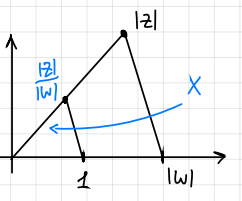
\includegraphics[]{images/4_36_division.png}
\end{center}

$$\frac{w}{1}=\frac{z}{x} \Rightarrow x = \frac{z}{w}$$

\par \Note Помним, что комплексное число можно построить тогда и только когда когда можно построить действительную и мнимую часть (билет 43 на уд), значит частное для них тоже можно построить (домножаем на сопряженное). Корень из комплексных чисел можем извлекать с помощью формулы Муавра (половинный угол мы можем построить)